\section{Reflection}
\subsection{Errors and Missing Features}
\begin{frame}{Reflection}{Errors and Missing Features}%+fault kode
	Error: removePassedMeals 
	\begin{itemize}
		\item Intention
			\begin{itemize}
			\item Remove ingredients from meals cooked
			\end{itemize}
		\item Error
			\begin{itemize}
			\item Incorrect amount of ingredients are removed
			\end{itemize}
		\item Consequence
			\begin{itemize}
			\item The inventory does not represent the reality
			\end{itemize}
	\end{itemize}
\end{frame}
\begin{frame}{Reflection}{Errors and Missing features}	
		Error: addValuesToSearch
		\begin{itemize}
			\item Intention
				\begin{itemize}
				\item Get relevant recipes
				\end{itemize}
			\item Error
				\begin{itemize}
				\item Comparisons between inventory and needed ingredients can be wrong 
				\end{itemize}
			\item Consequence
				\begin{itemize}
				\item Wrong presentation of recipes
				\end{itemize}
		\end{itemize}
\end{frame}

\begin{frame}{Reflection}{Errors and Missing Features}%+fault kode
	Error: settingsViewModel
	\begin{itemize}
		\item Intention
			\begin{itemize}
			\item The user can rate an ingredient
			\end{itemize}
		\item Error
			\begin{itemize}
			\item The in program names does not match
			\end{itemize}
		\item Consequence
			\begin{itemize}
			\item Incorrect representation of digits and the rating is not saved
			\end{itemize}
	\end{itemize}
\end{frame}
\begin{frame}{Reflection}{Errors and Missing features}	
		Missing feature: showMeals
		\begin{itemize}
			\item Intention
				\begin{itemize}
				\item Show the users meal plan for a given week
				\end{itemize}
			\item Functionality to change
				\begin{itemize}
				\item All meals on the database is shown, should only show logged in users meals
				\end{itemize}
			\item Benefit
				\begin{itemize}
				\item The user only sees relevant meal objects on their meal plan
				\end{itemize}
		\end{itemize}
\end{frame} %Anders over and out

\subsection{Optimisation}
\begin{frame}{Reflection}{Optimisation}
	Minimize communication between server and client
	\begin{itemize}
		\item Search
		\begin{itemize}
			\item .ToList()
		\end{itemize}
		\item Caching
		\begin{itemize}
			\item Save meals locally
			\item Local list of inventory
			\item Better allowance of off-line usage
		\end{itemize}
	\end{itemize}
\end{frame}

\subsection{Evaluation of Design}
\begin{frame}{Reflection}{Evaluation of Design}
	\begin{itemize}
		\item Scheduled meal page, update button
		\newline 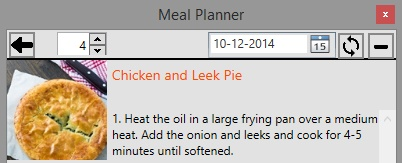
\includegraphics[scale=0.4]{./graphics/datepicker}
		\item Deleting meal
		\newline 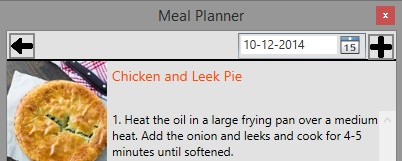
\includegraphics[scale=0.4]{./graphics/datepicker-not-planned}
	\end{itemize}
\end{frame}

\subsection{Requirements}
\begin{frame}{Reflection}{Requirements}%som er opfyldt/dem som ikke er.
	The two main problems:
	\begin{itemize}
		\item Planning and managing meals
		\item Minimizing food waste
	\end{itemize}	
	Problem based requirements:
	\begin{itemize}
		\item To much food being wasted
		\item Miscalculations happen in groups
		\item Shopping is time consuming
		\item Diets are difficult
		\item Consumers living alone have the most food waste
		\item Consumers living alone have a higher cost per meal
	\end{itemize}

\end{frame}
\begin{frame}{Reflection}{Requirements}%som er opfyldt/dem som ikke er.
The two main problems:
	\begin{itemize} \color{dkgreen}
		\item Planning and managing meals
		\item Minimizing food waste
	\end{itemize}
	Problem based requirements:
	\begin{itemize}
		\item {\color{dkgreen}To much food being wasted}
		\item {\color{red}Miscalculations happen in groups}
		\item {\color{orange}Shopping is time consuming}
		\item {\color{orange}Diets are difficult}
		\item {\color{orange}Consumers living alone have the most food waste}
		\item {\color{orange}Consumers living alone have a higher cost per meal}
	\end{itemize}
\end{frame}

\subsection{Future Improvements}
\begin{frame}{Reflection}{Future Improvements}
	\begin{itemize}
		\item Waterfall versus iterative
		\begin{itemize}
			\item run multiple tests
		\end{itemize}
		\item IDA or focus groups
		\item Other functionality
		\begin{itemize}
			\item Budget
			\item Diabetic
		\end{itemize}
	\end{itemize}
\end{frame}
